% Invariant patterns under "Kasami is Almost Bent".
% Build with a Unicode engine (tectonic recommended; arXiv supports xelatex too):
%   tectonic kasami-invariant-patterns.tex
% Lean snippets keep their real unicode, rendered with DejaVu Sans Mono.
\documentclass[11pt]{article}

\usepackage[margin=1.15in]{geometry}
\usepackage{amsmath,amssymb}
\usepackage{xcolor}
\usepackage{fontspec}
\usepackage{listings}
\usepackage{tikz}
\usepackage{tikz-cd}
\usepackage[most]{tcolorbox}
\usepackage{colortbl}
\usetikzlibrary{positioning,arrows.meta,fit,backgrounds,calc}

\usepackage{parskip}
\setlength{\parskip}{0.9em}
\linespread{1.12}

% Unicode fonts: a mono for Lean glyphs, a sans for little icons.
\newfontfamily\leanmono{DejaVu Sans Mono}[Scale=0.84]
\newfontfamily\dingfont{DejaVu Sans}

\newcommand{\ic}[1]{{\dingfont #1}}      % an icon glyph
\newcommand{\pencil}{\ic{✎}}
\newcommand{\bulb}{\ic{★}}
\newcommand{\spark}{\ic{✦}}
\newcommand{\hand}{\ic{☞}}

% --- Lean listing style --------------------------------------------------------
\definecolor{leanbg}{gray}{0.97}
\definecolor{leankw}{rgb}{0.30,0.20,0.65}
\definecolor{leancm}{rgb}{0.35,0.45,0.35}
\lstdefinestyle{lean}{
  backgroundcolor=\color{leanbg},
  basicstyle=\leanmono\small,
  keywordstyle=\color{leankw}\bfseries,
  commentstyle=\color{leancm}\itshape,
  morekeywords={def,theorem,lemma,structure,where,fun,Prop,Type,variable,
    namespace,end,open,noncomputable,Field,Fintype,CharP,Odd,Nat,import,
    Bijective,Function,by,intro,exact,have,convert,rw,simp,ext},
  morecomment=[l]{--},
  columns=fullflexible, keepspaces=true, showstringspaces=false,
  frame=single, framesep=6pt, xleftmargin=4pt,
  aboveskip=1.0em, belowskip=1.0em, extendedchars=true,
}
\lstset{style=lean}

% --- educational decoration boxes ---------------------------------------------
\newtcolorbox{bigidea}{colback=blue!4,colframe=blue!55!black,
  fonttitle=\bfseries, title={\bulb\ \ BIG IDEA}, sharp corners=south,
  boxrule=0.7pt, left=6pt,right=6pt,top=4pt,bottom=4pt}
\newtcolorbox{remarkbox}{colback=gray!6,colframe=gray!60!black,
  fonttitle=\bfseries, title={\pencil\ \ REMARK}, sharp corners=south,
  boxrule=0.6pt, left=6pt,right=6pt,top=4pt,bottom=4pt}
\newtcolorbox{coolfact}{colback=orange!7,colframe=orange!70!black,
  fonttitle=\bfseries, title={\spark\ \ COOL FACT}, sharp corners=south,
  boxrule=0.6pt, left=6pt,right=6pt,top=4pt,bottom=4pt}
% ------------------------------------------------------------------------------

\title{\bf Invariant Patterns under ``Kasami is Almost Bent''\\[3pt]
  \large Tiny atoms that propagate $\;$+$\;$ which ones warrant a categorical reading}
\author{}
\date{}

\begin{document}
\maketitle

\begin{abstract}\noindent
We collect the \emph{smallest} reusable lemmas under the Lean proof
``Kasami is Almost Bent'' and show they are all one idea wearing six costumes:

\[
  \boxed{\;\text{property } P \text{ is unchanged when we move along a symmetry}\;}
\]

In type theory / category theory this is \emph{transport along an iso}:
$P$ is a \textbf{fixed point} of an automorphism action, i.e.\ an \emph{invariant}.

We give each atom a formula, a picture, and the real Lean snippet
(file \texttt{Kasami/InvariantPatterns.lean}, fully proved, no \texttt{sorry}).
Then we read \texttt{FiniteField/Thm32.lean} and sort \emph{every} supporting
lemma into \textbf{functorial} vs \textbf{algebra / Galois / reindexing} ---
to see which actually deserve a categorical reading.
\end{abstract}

\bigskip

\begin{bigidea}
One symmetry $\;\Rightarrow\;$ one invariance lemma.
Stack the lemmas $\;\Rightarrow\;$ the headline theorem.

\[
  \underbrace{\text{Mathlib atoms}}_{\text{leaves}}
  \;\xrightarrow{\;\text{transport}\;}\;
  \underbrace{\text{Kasami is APN}}_{\text{pillar}}
  \;\xrightarrow{\;\text{transport}\;}\;
  \underbrace{\text{Kasami is AB}}_{\text{crown}}
\]
\end{bigidea}

% =====================================================================
\section{The shape: six atoms, one law}

A \emph{symmetry} is an iso $\sigma$.
An \emph{invariance lemma} says: $P(\sigma\!\cdot\! x)\iff P(x)$.

\begin{center}
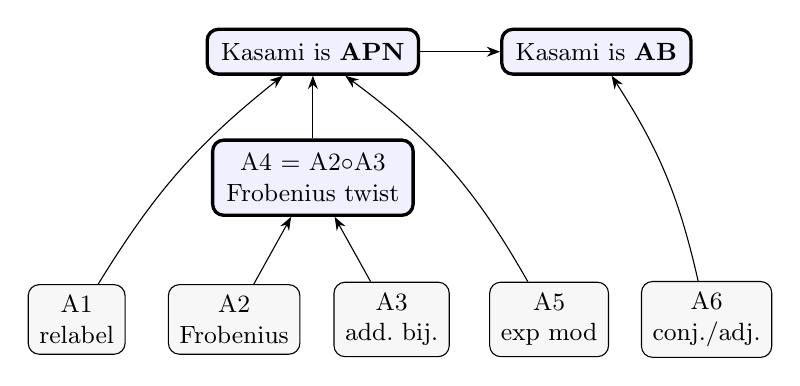
\begin{tikzpicture}[
  every node/.style={font=\small},
  atom/.style={draw,rounded corners,fill=leanbg,align=center,inner sep=4pt},
  hi/.style={draw,rounded corners,very thick,fill=blue!6,align=center,inner sep=5pt},
  >=Stealth ]
  \node[atom] (a1) at (-5.0,0) {A1\\ relabel};
  \node[atom] (a2) at (-3.0,0) {A2\\ Frobenius};
  \node[atom] (a3) at (-1.0,0) {A3\\ add.\ bij.};
  \node[atom] (a5) at ( 1.0,0) {A5\\ exp mod};
  \node[atom] (a6) at ( 3.0,0) {A6\\ conj./adj.};

  \node[hi] (a4) at (-2.0,1.8) {A4 = A2$\circ$A3\\ Frobenius twist};
  \node[hi] (apn) at (-2.0,3.4) {Kasami is \textbf{APN}};
  \node[hi] (ab)  at ( 1.6,3.4) {Kasami is \textbf{AB}};

  \draw[->] (a2)--(a4); \draw[->] (a3)--(a4);
  \draw[->] (a4)--(apn); \draw[->] (a5) to[bend right=12] (apn);
  \draw[->] (a1) to[bend left=10] (apn);
  \draw[->] (a6) to[bend right=10] (ab);
  \draw[->] (apn)--(ab);
\end{tikzpicture}
\end{center}

\begin{remarkbox}
Read bottom $\to$ top. Each arrow is ``transport along a symmetry''.
The \emph{same} five atoms reappear in \texttt{Lemma31}, \texttt{FrobAlg},
\texttt{KasamiEvenK}.
\end{remarkbox}

% =====================================================================
\section{Atom 1 --- relabel a parameter}

\textbf{Symmetry:} a bijection $\sigma$ on the index set.

\[
  \bigl(\forall a\neq b,\; R(\sigma a,\sigma b)\bigr)
  \;\Longleftrightarrow\;
  \bigl(\forall a\neq b,\; R(a,b)\bigr)
\]

A ``for all distinct pairs'' fact does not care how we \emph{name} the pairs.

\begin{lstlisting}
lemma forall_pairs_relabel {α : Type*} {σ : α → α} (hσ : Bijective σ)
    {R : α → α → Prop} :
    (∀ a b, a ≠ b → R (σ a) (σ b)) ↔ (∀ a b, a ≠ b → R a b)
\end{lstlisting}

\begin{center}
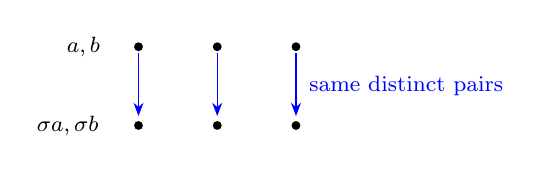
\begin{tikzpicture}[>=Stealth,every node/.style={font=\footnotesize}]
  \foreach \i in {0,1,2} { \fill (\i,1) circle (1.6pt); \fill (\i,0) circle (1.6pt);}
  \node at (-0.7,1) {$a,b$}; \node at (-0.9,0) {$\sigma a,\sigma b$};
  \foreach \i in {0,1,2} \draw[->,blue] (\i,0.92)--(\i,0.12);
  \node[blue] at (3.4,0.5) {same distinct pairs};
\end{tikzpicture}
\end{center}

\begin{coolfact}
This is \textbf{naturality} of the predicate $\forall\text{-pairs}$ along $\sigma$.
In \texttt{Lemma31} it slides the bijectivity test along the multiplicative
map $M$ (\texttt{forall\_ne\_bij}).
\end{coolfact}

% =====================================================================
\section{Atom 2 --- Frobenius is an additive automorphism}

\textbf{Symmetry:} $\;\phi_j(x)=x^{2^{j}}$ on $\mathrm{GF}(2^n)$.

\[
  \phi_j(x+y)=\phi_j x+\phi_j y
  \qquad\text{and}\qquad
  \phi_j\in\operatorname{Aut}(F,+).
\]

Freshman's dream in char $2$ $\Rightarrow$ additive; finite + injective
$\Rightarrow$ bijective.

\begin{lstlisting}
lemma frob_add (j : ℕ) (x y : F) :
    (x + y) ^ (2 ^ j) = x ^ (2 ^ j) + y ^ (2 ^ j)

lemma frob_bij (j : ℕ) : Bijective (fun x : F => x ^ (2 ^ j))
\end{lstlisting}

\begin{center}
\begin{tikzcd}[column sep=large]
F \arrow[r,"\phi_j"] \arrow[d,"+y"'] & F \arrow[d,"+\,\phi_j y"] \\
F \arrow[r,"\phi_j"'] & F
\end{tikzcd}
\end{center}

\begin{remarkbox}
Lean fact used: \texttt{add\_pow\_char\_pow} (Mathlib) and
\texttt{Finite.injective\_iff\_bijective}. This is the \emph{only} automorphism
the APN pillar needs.
\end{remarkbox}

% =====================================================================
\section{Atom 3 --- APN survives an additive bijection}

\textbf{Symmetry:} post-compose by an additive bijection $\sigma$.

\[
  \operatorname{IsAPN}(f)\;\Longrightarrow\;\operatorname{IsAPN}(\sigma\circ f).
\]

APN counts collisions of $f(x{+}a)+f(x)$. An additive \emph{bijection} keeps
collisions exactly, so the count is unchanged.

\begin{lstlisting}
lemma isAPN_comp_addBij {f σ : F → F} (hf : IsAPN f)
    (hbij : Bijective σ) (hadd : ∀ x y, σ (x + y) = σ x + σ y) :
    IsAPN (σ ∘ f)
\end{lstlisting}

\begin{center}
\begin{tikzcd}[column sep=2.2cm]
x \arrow[r,"\text{2-to-1 diff}"] \arrow[d,"f"'] & b \\
F \arrow[r,"\sigma\;(\cong)"'] & F \arrow[u,"\text{same count}"']
\end{tikzcd}
\end{center}

\begin{coolfact}
This is \emph{the} propagation pattern the user spotted: ``additive bijection''
travels from \texttt{FrobAlg}/Mathlib into \texttt{KasamiEvenK}.
APN is a \textbf{conjugation-invariant} of the additive group.
\end{coolfact}

% =====================================================================
\section{Atom 4 --- Frobenius exponent twist (A2 $\circ$ A3)}

Glue Atom 2 into Atom 3:

\[
  x^{\,d\cdot 2^{j}}=(x^{d})^{2^{j}}=\phi_j(x^{d})
  \qquad\Rightarrow\qquad
  \operatorname{IsAPN}(x^{d})\Rightarrow\operatorname{IsAPN}(x^{d\cdot 2^{j}}).
\]

\begin{lstlisting}
lemma isAPN_frob_twist {d : ℕ} (hf : IsAPN (fun x : F => x ^ d)) (j : ℕ) :
    IsAPN (fun x : F => x ^ (d * 2 ^ j))
\end{lstlisting}

\begin{center}
\begin{tikzcd}[column sep=1.6cm,row sep=small]
& x \arrow[dl,"x^{d}"'] \arrow[dr,"x^{d\cdot 2^{j}}"] & \\
x^{d} \arrow[rr,"\phi_j"'] & & x^{d\cdot 2^{j}}
\end{tikzcd}
\end{center}

\begin{bigidea}
A4 is the engine of \texttt{kasami\_apn\_of\_complement}: it lifts Kasami-APN
from a parameter $k$ to its complement $n-k$, with \emph{no parity restriction}.
APN is invariant along the \textbf{whole Frobenius orbit} of the exponent.
\end{bigidea}

% =====================================================================
\section{Atom 5 --- slide the exponent mod $|F|-1$}

\textbf{Symmetry:} $\mathbb{Z}/(|F|{-}1)$ acting on exponents (for $x\neq 0$).

\[
  a\equiv b \pmod{|F|-1}\;\Longrightarrow\;x^{a}=x^{b}.
\]

\begin{lstlisting}
lemma pow_invariant_mod {x : F} (hx : x ≠ 0) {a b : ℕ}
    (h : a % (Fintype.card F - 1) = b % (Fintype.card F - 1)) :
    x ^ a = x ^ b
\end{lstlisting}

\begin{center}
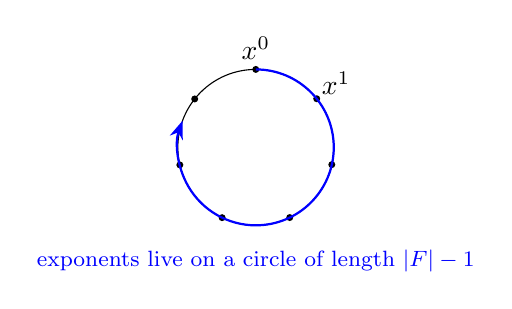
\begin{tikzpicture}[scale=0.9,>=Stealth]
  \def\R{1.1}\draw (0,0) circle (\R);
  \foreach \i in {0,...,6}{\fill (90-\i*51.4:\R) circle (1.4pt);}
  \node at (90:\R+0.3){$x^0$}; \node at (90-51.4:\R+0.35){$x^1$};
  \draw[->,blue,thick] (90:\R) arc (90:-200:\R);
  \node[blue] at (0,-1.6){\footnotesize exponents live on a circle of length $|F|-1$};
\end{tikzpicture}
\end{center}

\begin{remarkbox}
This is the wrap-around behind the Kasami congruence
$d_k\equiv d_{n-k}\cdot 2^{2k}\pmod{2^n-1}$ in \texttt{KasamiEvenK}.
\end{remarkbox}

% =====================================================================
\section{Atom 6 --- bijectivity is a conjugation invariant}

\textbf{Symmetry:} conjugate a self-map by an equivalence $e$.

\[
  \operatorname{Bijective}(e\circ f\circ e^{-1})
  \;\Longleftrightarrow\;
  \operatorname{Bijective}(f).
\]

\begin{lstlisting}
lemma bijective_conj_invariant {α β : Type*} (e : α ≃ β) (f : α → α) :
    Bijective (e ∘ f ∘ e.symm) ↔ Bijective f
\end{lstlisting}

\begin{center}
\begin{tikzcd}[column sep=large,row sep=large]
A \arrow[r,"f"] \arrow[d,"e"',"\cong"] & A \arrow[d,"e","\cong"'] \\
B \arrow[r,"e f e^{-1}"'] & B
\end{tikzcd}
\end{center}

\begin{coolfact}
The trace-adjoint $A\mapsto A^{*}$ in \texttt{Lemma31}
(\texttt{bijective\_iff\_adjoint\_bijective}) is exactly such a symmetry:
\textbf{duality} keeps bijectivity. ``Is it a permutation?'' is a self-dual
question.
\end{coolfact}

% =====================================================================
\section{How the atoms reach the crown}

\begin{center}
\begin{tikzcd}[column sep=1.4cm,row sep=large]
\text{A2}+\text{A3} \arrow[r,Rightarrow] & \text{A4} \arrow[dr,Rightarrow] & \\
\text{A5} \arrow[r,Rightarrow] & \text{A4 on }d_k \arrow[r,Rightarrow] & \boxed{\text{Kasami APN, all }k} \arrow[d,Rightarrow] \\
& & \boxed{\textbf{Kasami AB}}
\end{tikzcd}
\end{center}

The Lean synthesis is one line:

\begin{lstlisting}
theorem isAPN_invariant_along_frobenius_orbit {d : ℕ}
    (hf : IsAPN (fun x : F => x ^ d)) (j : ℕ) :
    IsAPN (fun x : F => x ^ (d * 2 ^ j)) :=
  isAPN_frob_twist hf j
\end{lstlisting}

% =====================================================================
\section{Reading \texttt{Thm32.lean}: functorial vs algebra / Galois / reindexing}

Theorem 3.2 (Dempwolff--Müller) proves $x\mapsto L(x)\,x^{k}$ is a permutation
of $\mathrm{GF}(2^n)$, with $L(x)=\sum_{i<m}x^{2^i}$ the truncated trace.

We sort \emph{every} supporting lemma into four bins.
Only the first bin warrants a categorical reading.

\begin{center}\small
\renewcommand{\arraystretch}{1.25}
\begin{tabular}{@{}p{4.7cm} p{3.1cm} p{4.6cm}@{}}
\hline
\textbf{lemma} & \textbf{bin} & \textbf{why} \\
\hline
\rowcolor{blue!7}
\texttt{truncTrace\_add},\ \texttt{\_zero} & \textbf{functorial} & $L$ is a morphism in $\mathbf{Ab}$ ($\mathtt{map\_add}$, $\mathtt{map\_zero}$) \\
\rowcolor{blue!7}
\texttt{dicksonF\_map\_ringHom} & \textbf{functorial} & naturality: $f_m$ commutes with \emph{every} ring hom ($\mathtt{map\_sum}$, $\mathtt{map\_pow}$) \\
\rowcolor{blue!7}
\texttt{LxXk'\_bijective} (adjoint swap) & \textbf{functorial} & trace-duality / adjunction (\texttt{adjoint\_swap\_bij}, \texttt{trace\_nondegenerate}) \\
\rowcolor{blue!7}
\texttt{LxXk\_bijective} (inj.\ part) & \textbf{functorial} & finite: $\mathrm{inj}\Leftrightarrow\mathrm{surj}$ (\texttt{Finite.injective\_iff\_surjective}) \\
\hline
\texttt{truncTrace\_sq\_add\_self} & algebra & Artin--Schreier identity $L^2{+}L=x^{2^m}{+}x$ \\
\texttt{truncTrace\_one\_eq\_one} & algebra & char-2 parity count \\
\texttt{sq\_eq\_self\_imp} & algebra & root count $x^2{=}x\Rightarrow x\in\{0,1\}$ \\
\texttt{dicksonF\_one},\ \texttt{\_recursion\_mul} & algebra & polynomial recursion \\
\texttt{dicksonF\_functional} & algebra & $f_m(z{+}z^{-1})$ functional eq. \\
\texttt{eq\_or\_eq\_inv\_of\_add\_inv\_eq} & algebra & fibres of $z\mapsto z{+}z^{-1}$ \\
\texttt{truncTrace\_sq\_mul\_inv\_eq\_dicksonF} & algebra & rearrange a finite sum \\
\hline
\texttt{frob\_fixed\_of\_truncTrace\_zero} & Galois & $\ker L\subseteq\operatorname{Fix}\phi_m$ \\
\texttt{truncTrace\_ker\_trivial} & Galois & fixed field of $\gcd$ Frobenius \\
\texttt{exists\_add\_inv\_rep} & Galois & base change to $\overline{F}$ \\
\texttt{frob\_2n\_eq\_self\_of\_quad\_root} & Galois & Frobenius descent of a root \\
\texttt{truncTrace\_adj\_frob} & Galois & Frobenius reindex of the trace \\
\hline
\texttt{coprime\_mersenne\_double'} & reindexing & $\gcd(2^a{-}1,2^b{-}1)=2^{\gcd(a,b)}{-}1$ \\
exponent mod $2^n{-}1$ slides & reindexing & $\mathbb{Z}/(2^n{-}1)$ arithmetic \\
\hline
\end{tabular}
\end{center}

\begin{bigidea}
\textbf{Verdict.} Out of $\sim$22 lemmas, only \textbf{four shapes} are genuinely
functorial:
\[
  \underbrace{L\ \text{additive}}_{\text{morphism in }\mathbf{Ab}}\;,\quad
  \underbrace{f_m\circ\text{hom}=\text{hom}\circ f_m}_{\text{natural transf.}}\;,\quad
  \underbrace{A\leftrightarrow A^{*}}_{\text{adjunction}}\;,\quad
  \underbrace{\mathrm{inj}\Leftrightarrow\mathrm{surj}}_{\text{finite-set invariant}}.
\]
Everything else is char-2 \textbf{algebra}, \textbf{Galois} descent, or
modular \textbf{reindexing} --- field-specific computation, \emph{not} category
theory.
\end{bigidea}

\begin{coolfact}
The four functorial lemmas are exactly the \emph{invariant atoms} of Part~I:
\[
  \text{additivity}\;\sim\;\text{A2/A3},\qquad
  \text{naturality}\;\sim\;\text{A1},\qquad
  \text{adjoint}\;\sim\;\text{A6}.
\]
So ``which lemmas warrant a categorical reading?'' has the same answer as
``which atoms are transport-along-an-iso?'' --- they are the load-bearing
\textbf{invariance} steps, while the algebra/Galois bulk supplies the one hard
input (a single map is a bijection).
\end{coolfact}

% =====================================================================
\section{One sentence to remember}

\begin{center}\large
\hand\ \ \emph{Six symmetries, six invariance lemmas, one crown ---
and only the \textbf{transport} steps are categorical.}
\end{center}

\end{document}
